The \tmview offers an alternative visualization of the scaffold tree, which is described in \subsecref{sec:scaffoldhunter:treegeneration}. The hierarchy defined by the scaffold tree is represented by nested rectangles, see \shortfigref{fig:treemap:example} for an example showing a small data set.

%
\begin{figure}[!htb]
\begin{centering}
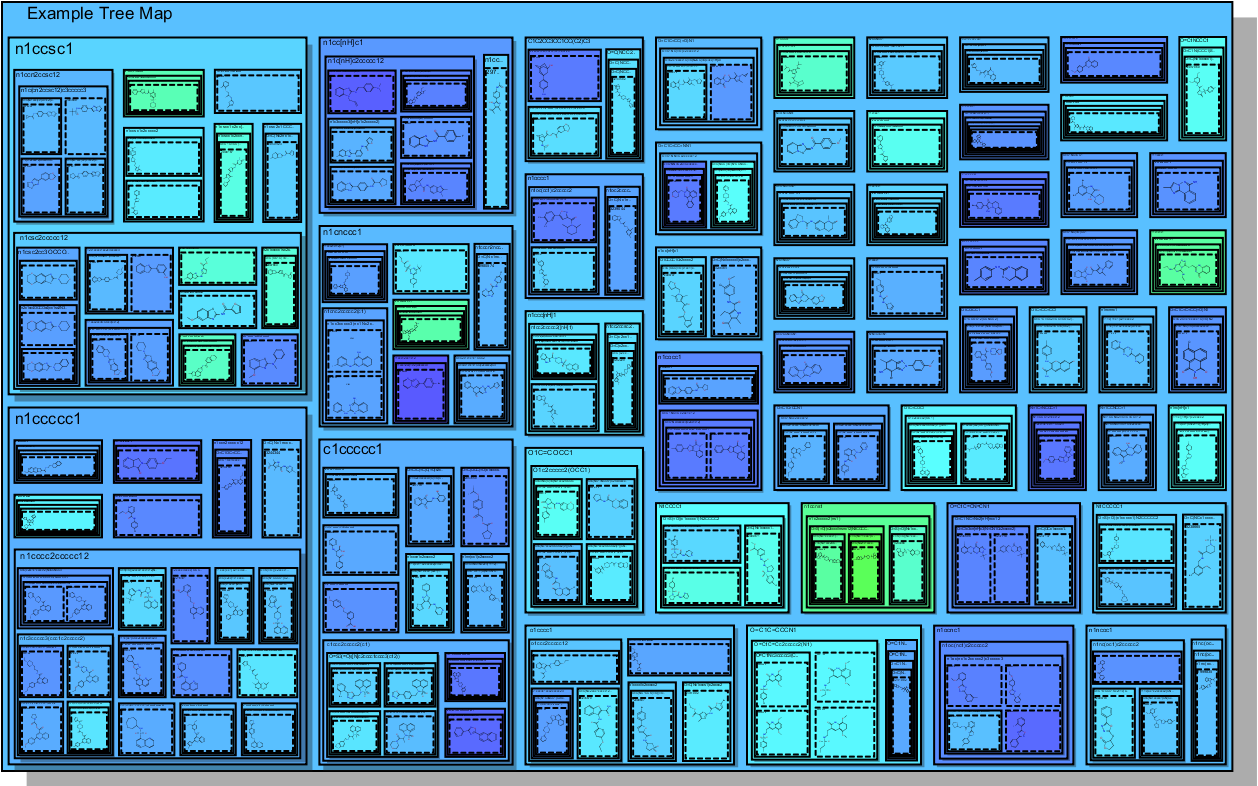
\includegraphics[width=0.8\columnwidth]{images/treemap/treemap_example}
\par\end{centering}

\caption{Example of a tree map}
\label{fig:treemap:example}

%
\end{figure}

\subsection{TreeMap \& Tool Bar}

The treemap itself allows you to zoom and pan around to get a detailed view for all parts of the tree map. This navigation works similar to the \stview. For zooming you can either use the mouse wheel, the buttons in the tool bar or the \gui{TreeMap} menu. To move around you can left-click into the tree map and move your mouse while keeping the left mouse button pressed. When you right-click a node in the tree map, the camera is centered around this node, so that the node fills out the whole screen. The detail increases on small zoom levels showing the title and image of nodes.

\subsection{Property Mappings}\label{sec:treemap:propertymapping}

Initially the tree map is plotted without colors and a uniform size for every molecule. The size and color of all nodes can be changed by assigning chemical properties to them. \shortfigref{fig:treemap:sidebar:mapping} shows the \gui{Property Mapping} panel, which is used for this purpose.

%
\begin{figure}[!htb]
\begin{centering}
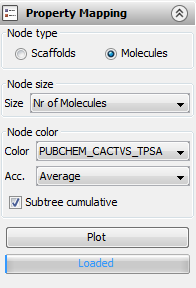
\includegraphics[scale=.6]{images/treemap/treemap_sidebar_mapping}
\par\end{centering}

\caption{Property Mapping panel}
\label{fig:treemap:sidebar:mapping}

%
\end{figure}

The individual options have the following functionality:

\begin{description}
\item[Node type] When \gui{Scaffolds} is selected only the scaffolds of the current subset are plotted. The option \gui{Molecules} additionally plots the molecules.
\item[Node size] Allows to map a chemical property to the node size. Only molecule properties can be mapped to the size, since the size of an inner nodes is always derived from its child nodes. Default is \gui{Nr of Molecules}.
\item[Node color] Allows to map a chemical property to the node color. The mapping can be combined with an accumulation function. This function works differently for molecule and scaffold properties:
\begin{itemize}
\item When using a molecule property, the accumulation function determines how to derive the colors of scaffolds from associated molecules. If \gui{Subtree cumulative} is enabled, the color of a scaffold is determined by the properties of all molecules that are contained in its subtree. If the option is disabled, only the molecules directly associated with the scaffold are considered.
\item When using a scaffold property and \gui{Subtree cumulative} is disabled, no accumulation is performed. If \gui{Subtree cumulative} is enabled, a scaffold combines its own color with its children's colors using the the function \gui{Acc.}.
\end{itemize}
If a property is not defined for a structure, it will be plotted in gray. 
\end{description}

\subsection{Color Legend}

The \gui{Legend} visualizes which property values have been mapped to which colors in the tree map. It is only visible, if a chemical property has been mapped to the node colors as explained in \subsecref{sec:treemap:propertymapping}. \shortfigref{fig:treemap:sidebar:legend} shows the legend for the tree map in \shortfigref{fig:treemap:example}.

%
\begin{figure}[!htb]
\begin{centering}
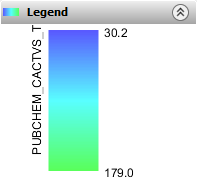
\includegraphics[scale=.6]{images/treemap/treemap_sidebar_legend}
\par\end{centering}

\caption{Color legend for the property mapping}
\label{fig:treemap:sidebar:legend}

%
\end{figure}

\subsection{Detail View}

The \gui{Detail View} shows additional information for a single scaffold or molecule. When you move the mouse cursor over a chemical structure in the tree map, an image and information about its size and color are displayed here.

%
\begin{figure}[!htb]
\begin{centering}
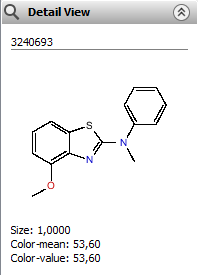
\includegraphics[scale=.6]{images/treemap/treemap_sidebar_detail}
\par\end{centering}

\caption{Detailed view for a single molecule}
\label{fig:treemap:sidebar:detail}

%
\end{figure}